E' compito degli \textit{Analisti} stilare il documento \textit{Analisi dei requisiti}.
In questo documento dovranno essere presenti tutti i requisiti ed i casi d'uso emersi dall'analisi del capitolato e dalle riunioni con il Proponente.\\

\subsection{Requisiti}

I requisiti dovranno essere classificati per tipo e priorità, utilizzando la seguente notazione:

R\{importanza\}\{tipo\}\{codice\}
\begin{itemize}
  \item Importanza può assumere i seguenti valori:
\begin{itemize}
	\item {OBB} : Requisito obbligatorio;
	\item {DES} : Requisito desiderabile;
	\item {OPZ} : Requisito opzionale.
\end{itemize}
  \item Tipo può assumere i seguenti valori:
\begin{itemize}
	\item {F} : Requisito funzionale;
	\item {Q} : Requisito di qualità;
	\item {P} : Requisito di prestazione;
	\item {V} : Requisito di vincolo.
\end{itemize}
  \item Codice rappresenta il codice univoco di ogni requisito in forma gerarchica.
\end{itemize}
Ogni requisito dovrà essere inserito (nel documento \textit{Analisi dei Requisiti}) in una tabella contenente il codice identificativo, una breve descrizione e la fonte.

\subsection{Casi d'uso}

Dopo la stesura dei requisiti è sempre compito degli analisti analizzare i casi d'uso (abbreviati con UC, use case).
Per ogni caso d'uso sono richieste le seguenti informazioni:
\begin{itemize}
	\item \textbf{Attori:} gli attori coinvolti nel caso d'uso (principali e secondari);
	\item \textbf{Scodo e descrizione:} una breve descrizione chiara e dettagliata del caso d'uso;
	%\item Codice identificativo: nel formato UCxx, dove xx indica un numero identificativo del caso d'uso;
	%\item Titolo: titolo sintetico del caso d'uso;
	\item \textbf{Precondizione:} la precondizione del requisito;
	\item \textbf{Flusso degli eventi:} specificare per ogni evento: descrizione, attori coinvolti e se lo scenario è descritto in dettaglio da un altro caso d'uso;
	%\item Diagramma: dovrà essere usato UML 2.4 per la creazione dei diagrammi dei casi d'uso;
	\item \textbf{Postcondizione:} la postcondizione del requisito.
\end{itemize}
\newpage
\subsection{Tracciamento}
Per il tracciamento dei requisiti è stato creato un database che tiene traccia dei requisiti, casi d'uso e tutte le dipendenze.
È stato realizzato un plugin per il Content Management System (CMS) WordPress per rendere possibile il popolamento e l'interrogazione.
Il plugin genera automaticamente il codice \LaTeX\ per l'\textit{Analisi dei Requisiti}.
Per sua natura, il plugin è portabile su tutte le versioni di WordPress ed alla fine del progetto sarà reso open-source in modo che possa essere riutilizzato da chi lo desideri. È stato scelto questo CMS poiché, essendo conosciuto da due membri del gruppo, permette di concentrarsi esclusivamente sulla gestione dei requisiti tralasciando tutti gli aspetti di contorno, comprimendo così notevolmente i tempi di sviluppo.
\begin{figure}[h]
\centering
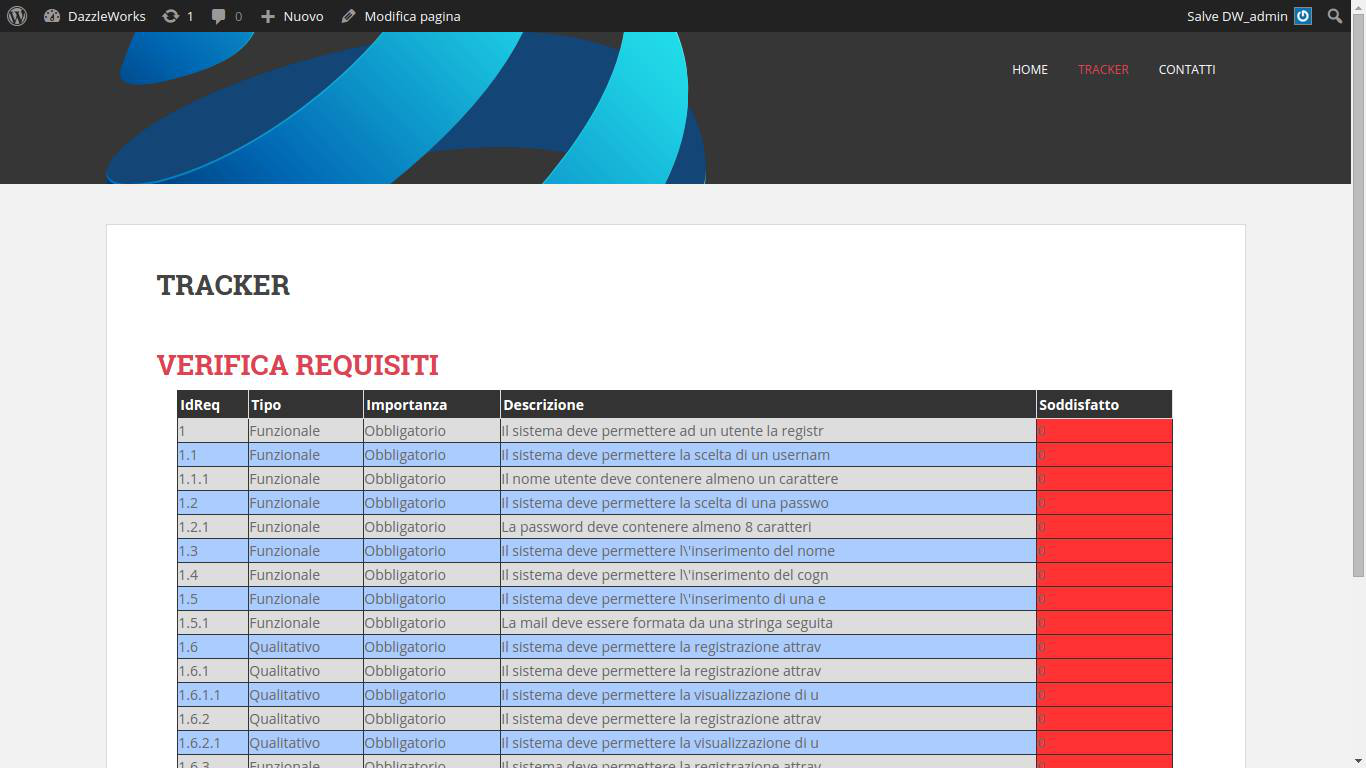
\includegraphics[width=0.7\linewidth]{img/tracker1}
\caption[Pagina riepilogo requisiti]{Pagina riepilogo requisiti}
\label{fig:tracker1}
\end{figure}
\begin{figure}[h]
\centering
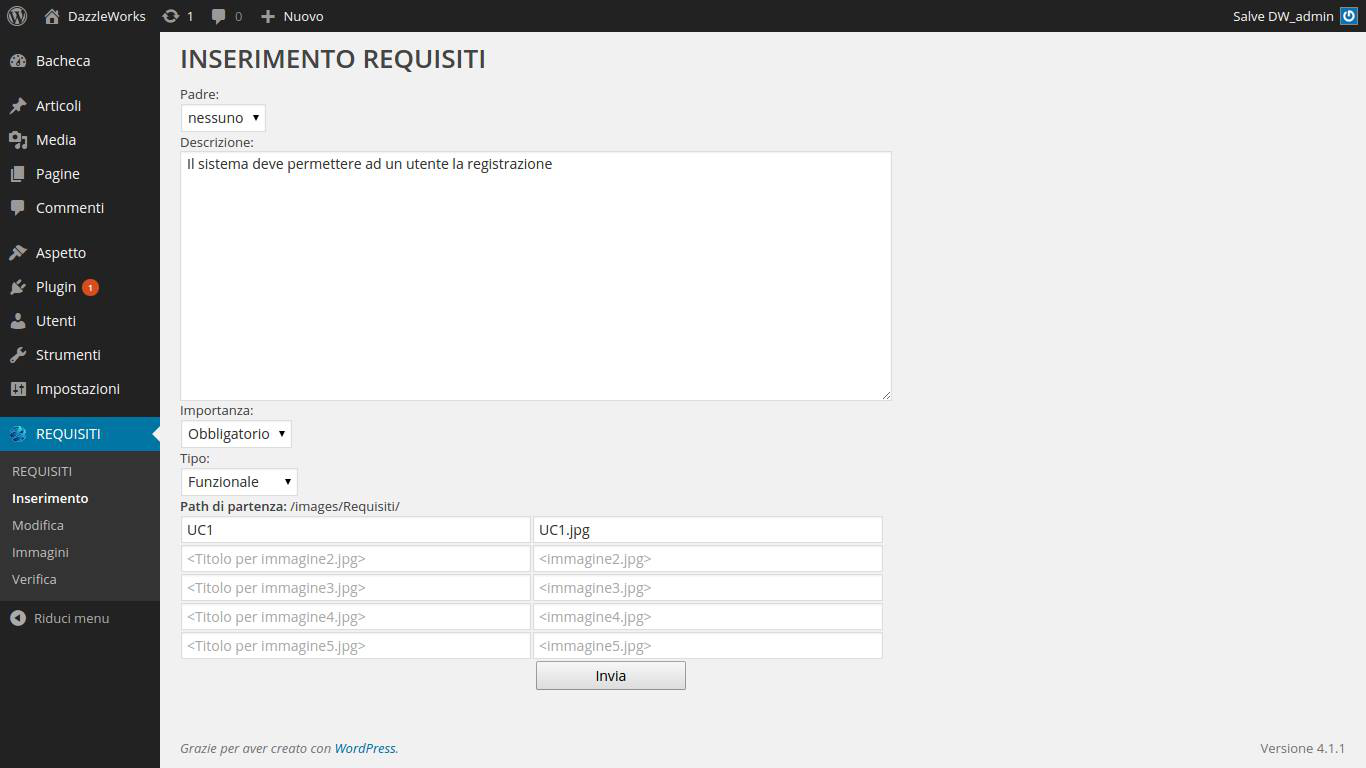
\includegraphics[width=0.7\linewidth]{img/tracker2}
\caption[Pagina inserimento requisito]{Pagina inserimento requisito}
\label{fig:tracker2}
\end{figure}

